% $Id: patches.tex 5678 2017-10-13 15:20:20Z mskala $

%
% MSK 010 patch suggestions
% Copyright (C) 2017  Matthew Skala
%
% This program is free software: you can redistribute it and/or modify
% it under the terms of the GNU General Public License as published by
% the Free Software Foundation, version 3.
%
% This program is distributed in the hope that it will be useful,
% but WITHOUT ANY WARRANTY; without even the implied warranty of
% MERCHANTABILITY or FITNESS FOR A PARTICULAR PURPOSE.  See the
% GNU General Public License for more details.
%
% You should have received a copy of the GNU General Public License
% along with this program.  If not, see <http://www.gnu.org/licenses/>.
%
% Matthew Skala
% https://northcoastsynthesis.com/
% mskala@northcoastsynthesis.com
%

\chapter{Patch Suggestions}

Use the MSK~010 as a modulation source for a classical analog oscillator;
here, it controls exponential FM and pulse width.

{\hspace*{\fill}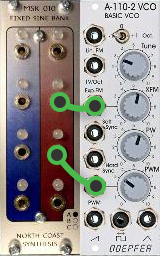
\includegraphics[scale=0.8]{patch1.png}\hspace*{\fill}\par} 

For modules that don't have built-in attenuators, it can be useful to run
the outputs through an external attenuator like the Triatt.  The Clouds is a
good candidate for modulation with the MSK~010 because it has many different
control voltage inputs; you might even want more than one MSK~010 to take
full advantage of it.

{\hspace*{\fill}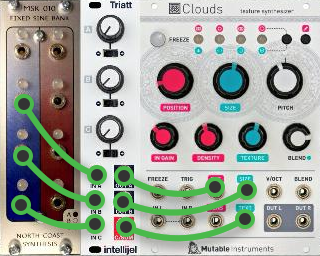
\includegraphics[scale=0.8]{patch2.png}\hspace*{\fill}\par} 

\newpage

A small amount of sine modulation on a BBD's clock gives a sound much
like an unstable tape recording.

{\hspace*{\fill}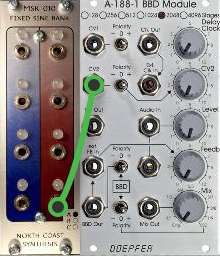
\includegraphics[scale=0.8]{patch3.png}\hspace*{\fill}\par} 

Mix slow sine waves and run them through a quantizer for an
automatically-generated but non-random melody.

{\hspace*{\fill}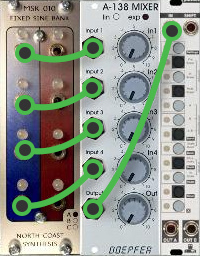
\includegraphics[scale=0.8]{patch4.png}\hspace*{\fill}\par} 
